\documentclass[UTF8]{ctexart}
\usepackage{enumerate}
\usepackage{amssymb}
\usepackage{graphicx}
\usepackage{subfigure}
\usepackage{amsmath}
\usepackage{geometry}
 \usepackage{indentfirst} 
\begin{document}
	\title{\textbf{《数据可视化》课程实践报告}\\[1ex]
	\begin{large}
		《倚天屠龙记》的文本分析及可视化
		\end{large}}
	\author{姓名:蒋慧\,\,学号:51194501050\,\,专业:软件工程\,\,组名:文本可视化}
	\maketitle

\section{引言}
\par{
	数据可视化主要旨在借助于图形化手段,清晰有效地传达与沟通信息。为了有效地传达思想概念,美学形式与功能需要齐头并进,
	通过直观地传达关键的方面与特征,从而实现对于相当稀疏而又复杂的数据集的深入洞察。
数据可视化与信息图形、信息可视化、科学可视化以及统计图形密切相关。当前,在研究、教学和开发领域,数据可视化乃是一个极为
活跃而又关键的方面。
}
\par{数据可视化就是一个
处于不断演变之中的概念,其边界在不断地扩大;因而,最好是对其加以宽泛的定义。
数据可视化指的是技术上较为高级的技术方法,而这些技术方法允许利用图形、图像处理、计算机视觉以及用户界面,通过表达
、建模以及对立体、表面、属性以及动画的显示,对数据加以可视化解释。与立体建模之类的特殊技术方法相比,数据可视化所涵
盖的技术方法要广泛得多。}
\section{相关工作}
\par{
	我的小组是做文本可视化,文本可视化在我的理解就是文字表达的内容和规律以视觉符号的形式表达出来,同时向人们提供与视
	觉信息进行快速交互的功能,使人们能够利用与生俱来的视觉感知的并行化处理能力快速获取大数据中所蕴含的的关键信息。
	文本数据可视化主要包含信息收集、数据预处理、知识表示、视觉呈现和交互等过程。文本可视化依赖于自然语言处理,因此词袋模型、
	命名实体识别、关键词抽取、主题分析、情感分析等是较常用的文本分析技术。文本分析的过程主要包括特征提取,通过分词、
	抽取、归一化等操作提取出文本词汇及的内容;利用特征构建向量空间模型并进行降维,以便将其呈现在低维空间,或者利用
	主题模型处理特征;最终以灵活有效的形式表示这些过程处理过的数据,以便进行可视化呈现和交互。
}
\section{问题描述}
\par{由于我和我的组员都不是可视化方向的,所以在开始进行这个大作业之前,我们都挺迷茫,而且觉得自己能力不够做不出来,但是在一步步摸索之后我们
发现了另一番天地。在此次实验中我们遇到的问题主要有一下几个方面:
}
\begin{enumerate}[(1)]
	\item 选题问题,我们了解了我们所做的文本可视化之后,发现我们组的东西技术难度不大,分析老师的要求之后,我们明白,技术不是问题,因为现在已经有很多成熟的工具可以帮助我们实现,所以我们主要应该选题和角度新颖有趣。
	\item 关键词提取,起初我们人为统计了大量的关键词比如人名,最后发现由于关键词太多反而影响最后出来的效果,人物关系可视化后比较冗杂没有意义。
	\item 中文问题,由于中文环境,给分词数据带来问题,编码不一样也会导致python读出来的数据有问题。
\end{enumerate}
\section{方案及实现}
\par{
根据我们组内细致的分工,我和另一个组员负责进行人物关系可视化部分,我们利用python的jieba分词库进行分词,但是需要我们提供给他主要人物名字以及
别名。gephi是一个开源的复杂网络数据可视化软件,可用于探索数据分析、链路分析、社交网络分析、生物网络分析等。我们需要把数据处理成gephi
可接受的csv格式,然后再进行绘制。我们的步骤如下
\begin{figure}[h]
	\centering
	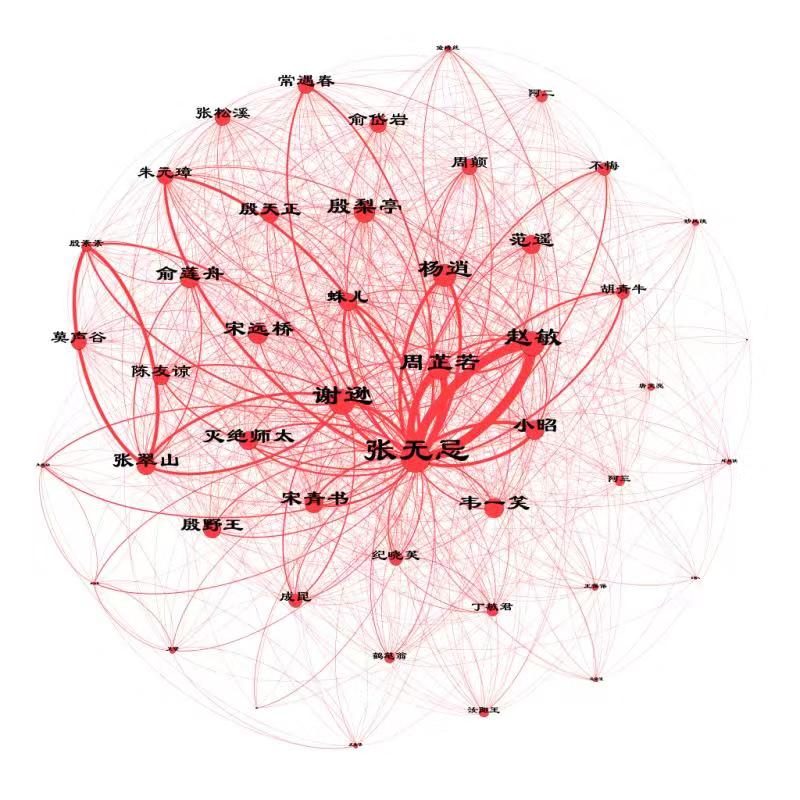
\includegraphics[width=5cm,height=5cm]{/Users/jiangqianxi/Desktop/github/Quantum-Computation-and-Quantum-Information/DataVisulization/政治小论文/WechatIMG22.jpeg }
	\caption{人物关系图}
	\end{figure}
\begin{enumerate}[(1)]
	\item 对文本进行针对性分词,统计人物在本文中的出场次数。
	\item 以段落为单位进行划分,统计每段中的人物,两两配对后计数,形成粗略的人物关系统计。
	\item 数据为gephi特定的csv格式,人物出场次数输出为格式为(Id,Label,Weight),人物关系输出格式为(Source,Target,Weigh)。这也就是之前所说的,用来绘制图的节点和边数据。
	\item 将文件导入gephi一键绘图,最后调整参数,让图具有良好的可视性。最后我们的得到的人物关系图如图1所示。
\end{enumerate}

}
\par{

}
\section{课程总结}
\par{
	通过这次课程,我觉得老师是很有趣,课代表也很有趣很机灵,想方设法引起大家的注意,
	但是总感觉无法集中注意力,我觉得是自己现在有点浮躁,既然进入研究生阶段就应该好好沉下心来
	做研究,期望这个阶段能好好完成,顺利毕业,适逢寒假将至,我打算利用这个寒假让自己完成自己的过渡。
	想清楚自己的方向目标,最近真是有点迷茫通过老师的言行,我感觉老师是一个很和蔼,没有架子的老师,很亲民。
	但是我个人觉得老师讲的东西太宽泛了,感觉是科普性质的课程。而且讲论文的意义我不是很明白,每个人上去讲论文,
	其他同学在下面也没听,就感觉浪费了很多时间。虽然是其他同学主动不听,这个真是没想到好的办法。我觉得其他同学不
	听可能是觉得自己不是这个方向的,然后学了也是但当涉猎,后面不知道什么时候用到,
	但是我觉得现在学了的东西以后总有机会用到,还是应该好好学习。
}
% ---- Bibliography ----
\bibliographystyle{unsrt}
\bibliography{cite}

\end{document}